\section*{Łączenie wyjaśnień różnych metod}
W tej sekcji przanalizujemy połączenie wyjaśnień generowanych przez różne matody XAI: LIME, SHAP i GradCAM.
Celem jest sprawdzenie, czy łączenie tych metod może dostarczyć bardziej szczegółowych lub ogólnych wyjaśnień.
Przeprowadzimy analizę na całym zbiorze danych, porównując wyniki uzyskane z połączenia wyjaśnień przez część wspólną oraz sumę obszarów

\subsection*{Część wspólna}
\begin{figure}
	\centering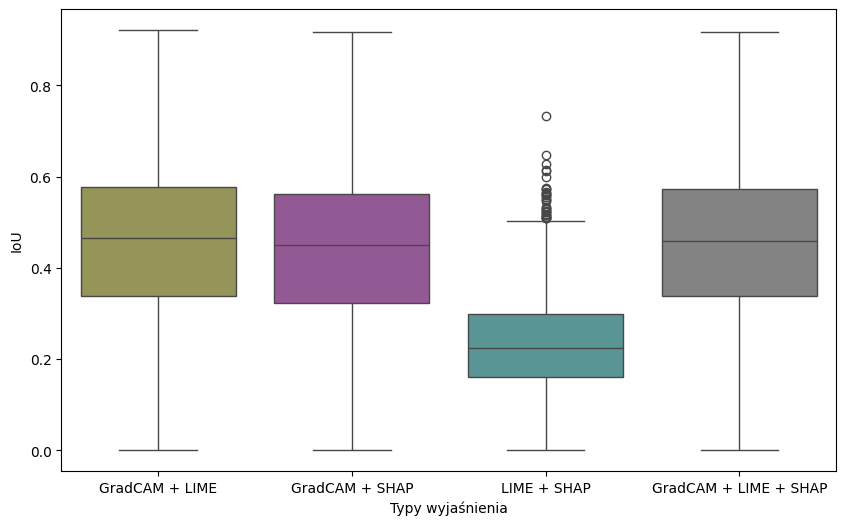
\includegraphics[width=.6\textwidth]{img/combine_iou_or}
	\caption{IoU}  \label{rys:combine_iou_or}
\end{figure}
\begin{figure}
	\centering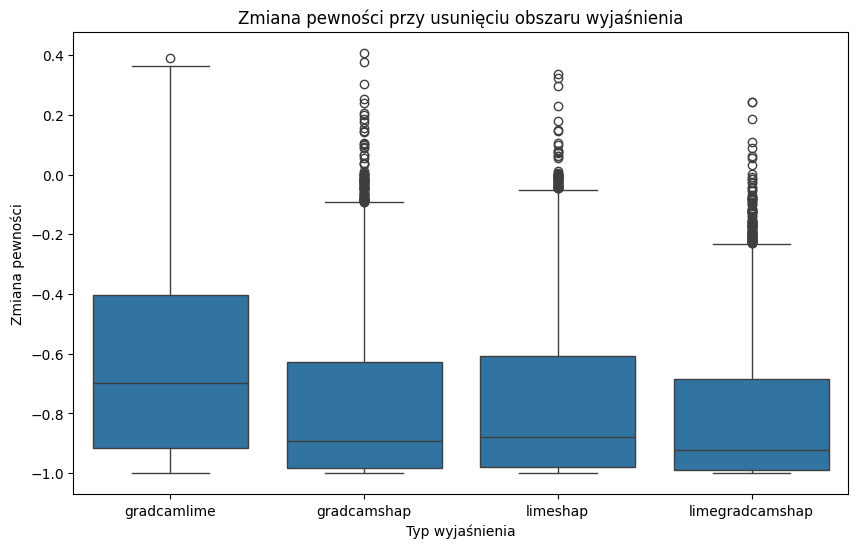
\includegraphics[width=.6\textwidth]{img/combine_confidence_mask_or}
	\caption{Zmiana pewności przy usunięciu obszarów wyjaśnienia}  \label{rys:combine_confidence_mask_or}
\end{figure}
\begin{figure}
	\centering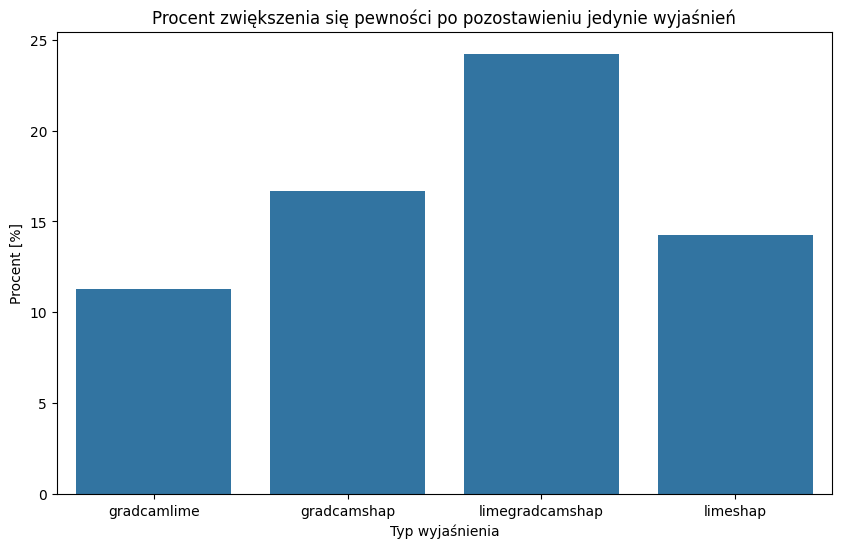
\includegraphics[width=.6\textwidth]{img/combine_confidence_womask_or}
	\caption{Procent zwiększenia się pewności po pozostawieniu jedynie obszarów wyjaśnień}  \label{rys:combine_confidence_womask_or}
\end{figure}

\subsection*{Suma obszarów}
\begin{figure}
	\centering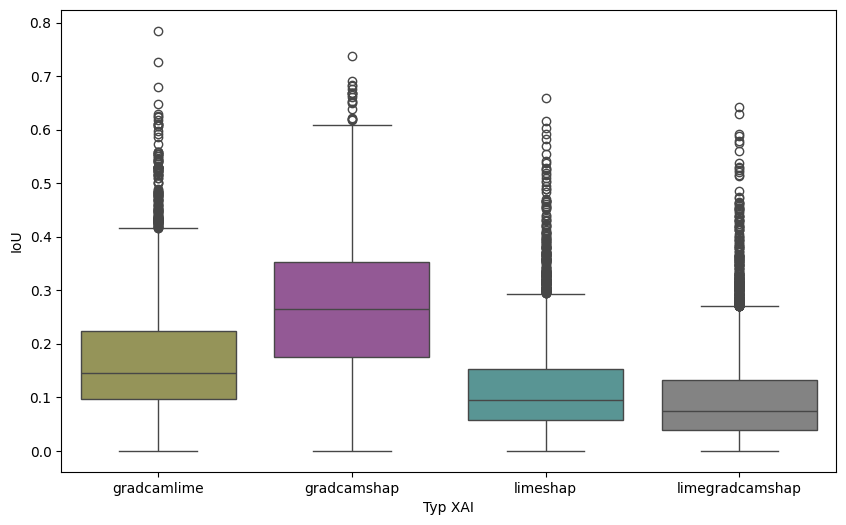
\includegraphics[width=.6\textwidth]{img/combine_iou_and}
	\caption{IoU}  \label{rys:combine_iou_and}
\end{figure}
\begin{figure}
	\centering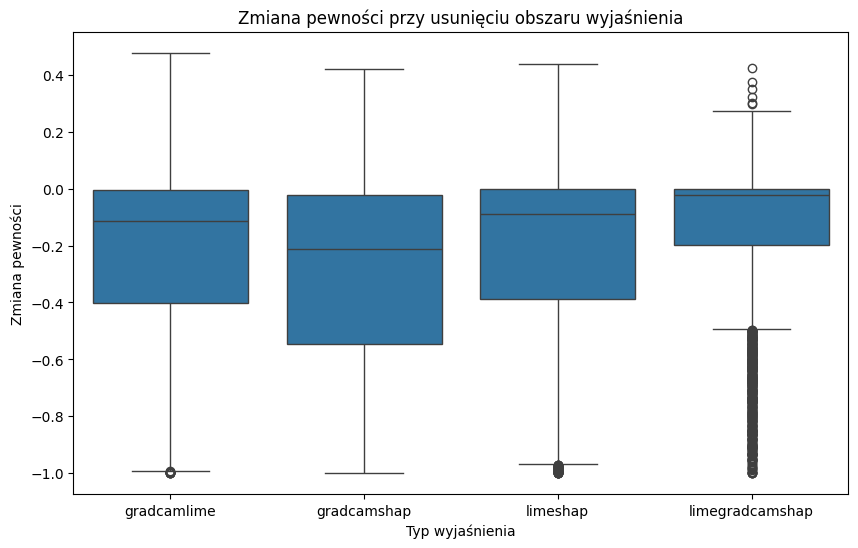
\includegraphics[width=.6\textwidth]{img/combine_confidence_mask_and}
	\caption{Zmiana pewności przy usunięciu obszarów wyjaśnienia}  \label{rys:combine_confidence_mask_and}
\end{figure}
\begin{figure}
	\centering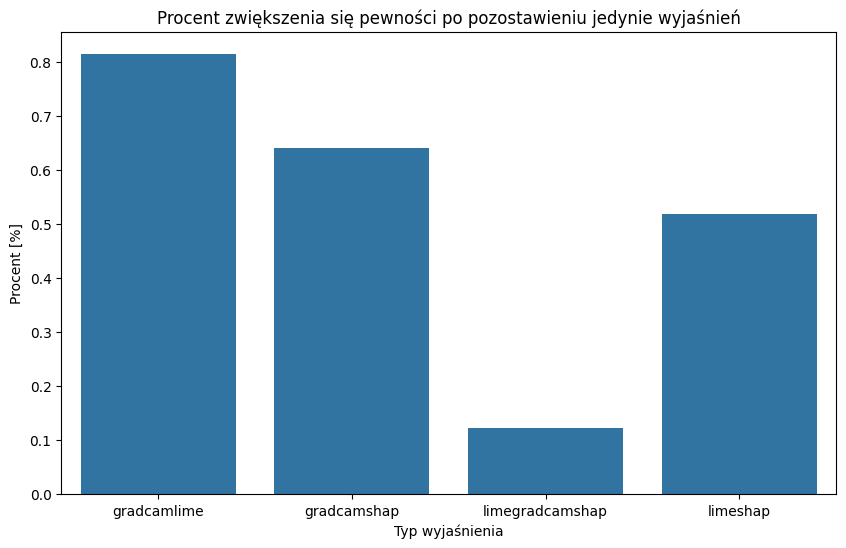
\includegraphics[width=.6\textwidth]{img/combine_confidence_womask_and}
	\caption{Procent zwiększenia się pewności po pozostawieniu jedynie obszarów wyjaśnień}  \label{rys:combine_confidence_womask_and}
\end{figure}

